\documentclass[12pt,a4paper]{article}

% --- Настройка языка и шрифтов для LuaLaTeX ---
\usepackage{fontspec}
\defaultfontfeatures{Ligatures=TeX,Scale=MatchLowercase}

\setmainfont{Alice-Regular}[
    Path=font/,
    Extension=.ttf,
    BoldFont = Alice-Regular,
    ItalicFont = Alice-Regular,
    BoldItalicFont = Alice-Regular,
    BoldFeatures = {FakeBold=1.6},
    ItalicFeatures = {FakeSlant=0.2},
    BoldItalicFeatures = {FakeBold=1.6,FakeSlant=0.2}
]

\newfontfamily\cyrillicfont{Alice-Regular}[
    Path=font/,
    Extension=.ttf,
    BoldFont = Alice-Regular,
    ItalicFont = Alice-Regular,
    BoldItalicFont = Alice-Regular,
    BoldFeatures = {FakeBold=1.6},
    ItalicFeatures = {FakeSlant=0.2},
    BoldItalicFeatures = {FakeBold=1.6,FakeSlant=0.2}
]

\usepackage{polyglossia}
\setmainlanguage{russian}
\setsansfont{TeX Gyre Heros}
\setmonofont{TeX Gyre Cursor}

\usepackage{graphicx}        					          % Графика
\usepackage[protrusion=false]{microtype}       	% Микротипографика
\usepackage{amsmath, amsfonts, amssymb, amsthm}	% Математика
\usepackage{braket} 							              % Braket нотация для квантовой механики
\usepackage{unicode-math} 						          % Современный пакет для математики в LuaLaTeX
\usepackage{longtable}       					          % Таблицы с разрывом страниц
\usepackage{tikz}           					          % Рисование
\usepackage[europeanresistors]{circuitikz}		  % Рисование электрических схем в европейском стиле
\usepackage{listings}							              % Для отображения кода
\usepackage{tabularx}       					          % Для таблиц во всю ширину
\usepackage{array}		  						            % Для расширенных возможностей таблиц
\usepackage{float}          					          % Для точного позиционирования фигур
\usepackage{pgfplots}                           % Для построения графиков
\usepackage{caption}                            % Для настройки подписей к рисункам и таблицам
\usepackage{xfp}                                % Для вычислений в LaTeX
\pgfplotsset{compat=1.18}
\usepackage[a4paper,left=20mm,right=20mm,top=20mm,bottom=20mm]{geometry}

\usetikzlibrary{arrows.meta}

% --- Колонтитулы ---
\usepackage{fancyhdr}
\pagestyle{fancy}
\fancyhf{}

\renewcommand{\headrulewidth}{0.4pt}
\renewcommand{\footrulewidth}{0.4pt}
\renewcommand\lstlistingname{Исходный код}

\lstdefinestyle{main}{
	backgroundcolor=\color{gray!8},   
	commentstyle=\color{green!50!black},
	keywordstyle=\color{blue!80!black},
	numberstyle=\small\color{darkgray},
	stringstyle=\rmfamily\color{orange!90!black},
	basicstyle=\ttfamily\small,
	breakatwhitespace=false,         
	breaklines=true,                   
	keepspaces=true,                 
	numbers=left,                    
	numbersep=8pt,                  
	showspaces=false,                
	showstringspaces=false,
	showtabs=false,                  
	tabsize=4
}	

\lstset{style=main}

\newcolumntype{C}{>{\centering\arraybackslash}X}
\renewcommand{\arraystretch}{1.25}

% =========================================================
%         СЛУЖЕБНЫЕ КОМАНДЫ ДЛЯ ВЫЧИСЛЕНИЙ
% =========================================================
\newcommand{\CalcZero} [1]{\fpeval{round((#1),0)}}
\newcommand{\CalcOne}  [1]{\fpeval{round((#1),1)}}
\newcommand{\CalcTwo}  [1]{\fpeval{round((#1),2)}}
\newcommand{\CalcThree}[1]{\fpeval{round((#1),3)}}
\newcommand{\CalcFour} [1]{\fpeval{round((#1),4)}}
\newcommand{\CalcFive} [1]{\fpeval{round((#1),5)}}

% ---------------------------------------------------------
% ОБЩИЕ ДАННЫЕ
% ---------------------------------------------------------
\def\VariantN{6}          					         % Номер варианта
\def\LabNumber{2}							               % Номер лабораторной работы
\def\LabTitle{Контрольная работа}                  % Название работы
\def\Discipline{Теория вероятности}				           % Название дисциплины

\title{
	МИНОБРНАУКИ РОССИИ

	федеральное государственное автономное образовательное учреждение

	высшего образования

	«Национальный исследовательский университет
	«Московский институт электронной техники»
	\vspace{2em}
}
\author{
}
\date{}

\begin{document}

\maketitle
\thispagestyle{fancy}

\begin{center}
\Large Контрольная работа $\LabNumber$
\end{center}

\begin{center}
\Large Вариант \VariantN
\end{center}

\vspace{12em}

\cfoot{Москва 2026}

\pagebreak

\fancyhead[L]{\LabTitle} 
\fancyhead[R]{\Discipline}
\fancyfoot[C]{\thepage}

\noindent$1.$ СВНТ $X$ имеет функцию распределения:
\[
F_X(x) =
\begin{cases}
	0 & x \leq -1 \\
	A(x + 1)^3 & -1 < x \leq 1 \\
	1 & x > 1
\end{cases}
\]
Найти $A$, вероятность попадания СВ $X$ в интервал $(-0{,}5; 0{,}5)$
и математическое ожидание СВ $X$.

\begin{center}

\begin{tikzpicture}
	% параметры
	\def\W{\textwidth} % ширина прямоугольника
	\def\H{41 * 5mm}   % высота прямоугольника
	\def\R{4mm}        % радиус скругления
	\def\S{5mm}        % шаг сетки

	% обрезаем всё по прямоугольнику со скруглёнными углами
	\begin{scope}
		\clip[rounded corners=\R] (0,0) rectangle (\W,\H);

		% тетрадная сетка
		\draw[step=\S, thin, gray!50] (0,0) grid (\W,\H);
	\end{scope}

	% внешний контур
	\draw[rounded corners=\R, gray] (0,0) rectangle (\W,\H);
\end{tikzpicture}
\end{center}

\noindent$2.$ Плотность распределения $f_X(x)$ СВНТ $X$ представлена на графике.
Найти $m_X$.

\begin{center}
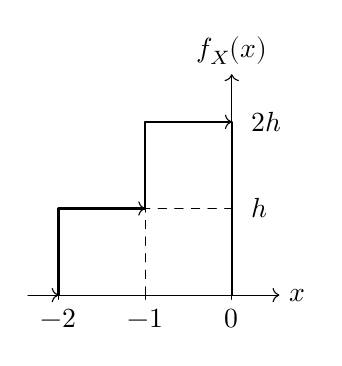
\begin{tikzpicture}[scale=1.1, line cap=round, line join=round]
	% Оси
	\draw[->] (-2.35,0) -- (0.55,0) node[right] {$x$};
	\draw[->] (0,0) -- (0,2.55) node[above] {$f_X(x)$};

	% Деления на оси x
	\foreach \x/\lab in {-2/$-2$, -1/$-1$, 0/$0$} {
		\draw (\x,0.05) -- (\x,-0.05);
		\node[below] at (\x,-0.05) {\lab};
	}

	% Уровни h и 2h
	\draw[dashed] (-2,1) -- (0,1);
	\draw[dashed] (-1,0) -- (-1,1);

	\node[right] at (0.12,1) {$h$};
	\node[right] at (0.12,2) {$2h$};

	% Плотность: от -2 до -1 высота h, от -1 до 0 высота 2h
	\draw[thick] (-2,0) -- (-2,1) -- (-1,1) -- (-1,2) -- (0,2) -- (0,0);

	% Стрелки-указатели уровней
	\draw[->] (-2.35,0) -- (-2,0);
	\draw[->] (-2,1) -- (-1,1);
	\draw[->] (-1,2) -- (0,2);
\end{tikzpicture}
\end{center}

\begin{center}

\begin{tikzpicture}
	% параметры
	\def\W{\textwidth} % ширина прямоугольника
	\def\H{40 * 5mm}   % высота прямоугольника
	\def\R{4mm}        % радиус скругления
	\def\S{5mm}        % шаг сетки

	% обрезаем всё по прямоугольнику со скруглёнными углами
	\begin{scope}
		\clip[rounded corners=\R] (0,0) rectangle (\W,\H);

		% тетрадная сетка
		\draw[step=\S, thin, gray!50] (0,0) grid (\W,\H);
	\end{scope}

	% внешний контур
	\draw[rounded corners=\R, gray] (0,0) rectangle (\W,\H);
\end{tikzpicture}
\end{center}

\noindent$3.$ Случайная величина $X \sim \mathbf{N}(6; 5)$.
Найти вероятность того, что СВ $X$ отклонится от своего математического ожидания
менее, чем на $1$.

\begin{center}

\begin{tikzpicture}
	% параметры
	\def\W{\textwidth} % ширина прямоугольника
	\def\H{47 * 5mm}   % высота прямоугольника
	\def\R{4mm}        % радиус скругления
	\def\S{5mm}        % шаг сетки

	% обрезаем всё по прямоугольнику со скруглёнными углами
	\begin{scope}
		\clip[rounded corners=\R] (0,0) rectangle (\W,\H);

		% тетрадная сетка
		\draw[step=\S, thin, gray!50] (0,0) grid (\W,\H);
	\end{scope}

	% внешний контур
	\draw[rounded corners=\R, gray] (0,0) rectangle (\W,\H);
\end{tikzpicture}
\end{center}

\noindent$4.$ Контрольную работу по теории вероятностей с первого раза успешно
выполняют $40\%$ студентов. Найти вероятность того, что из $400$ студентов
работу успешно выполнят не более $140$ студентов.

\begin{center}

\begin{tikzpicture}
	% параметры
	\def\W{\textwidth} % ширина прямоугольника
	\def\H{47 * 5mm}   % высота прямоугольника
	\def\R{4mm}        % радиус скругления
	\def\S{5mm}        % шаг сетки

	% обрезаем всё по прямоугольнику со скруглёнными углами
	\begin{scope}
		\clip[rounded corners=\R] (0,0) rectangle (\W,\H);

		% тетрадная сетка
		\draw[step=\S, thin, gray!50] (0,0) grid (\W,\H);
	\end{scope}

	% внешний контур
	\draw[rounded corners=\R, gray] (0,0) rectangle (\W,\H);
\end{tikzpicture}
\end{center}

\end{document}